% !TeX program = xelatex
\documentclass[3pt,landscape]{article}
\usepackage{multicol, calc, ifthen, amsmath, amsthm, amsfonts, amssymb, color, graphicx, hyperref, fontspec, xunicode}

\usepackage[landscape]{geometry}

\defaultfontfeatures{Mapping=tex-text,Scale=MatchLowercase}
\ifthenelse{\lengthtest { \paperwidth = 11in}}
    { \geometry{top=.3in,left=.3in,right=.3in,bottom=.3in} }
    {\ifthenelse{ \lengthtest{ \paperwidth = 297mm}}
        {\geometry{top=1cm,left=1cm,right=1cm,bottom=1cm} }
        {\geometry{top=1cm,left=1cm,right=1cm,bottom=1cm} }
    }
\pagestyle{empty}
\makeatletter
\setmainfont{Source Sans Pro}
\setmonofont{Menlo}
\DeclareMathSizes{3}{3}{2}{1}

\renewcommand{\section}{\@startsection{section}{1}{0mm}{-1ex plus -.5ex minus -.2ex}{0.5ex plus .2ex}{\normalfont\large\bfseries}}
\renewcommand{\subsection}{\@startsection{subsection}{2}{0mm}{-1explus -.5ex minus -.2ex}{0.5ex plus .2ex}{\normalfont\normalsize\bfseries}}
\renewcommand{\subsubsection}{\@startsection{subsubsection}{3}{0mm}{-1ex plus -.5ex minus -.2ex}{1ex plus .2ex}{\normalfont\small\bfseries}}
\makeatother
\setcounter{secnumdepth}{0}
\setlength{\parindent}{0pt}
\setlength{\parskip}{0pt plus 0.5ex}
\hypersetup{colorlinks=true, urlcolor=blue}
\def\ci{\perp\!\!\!\perp}

%%%%%%%%%%%%%%%%%%%%%%%%%%%%%%%%%%%%%%%%%%%%%%%%%%

\begin{document}
\raggedright
\footnotesize

\begin{multicols}{3}
\setlength{\premulticols}{1pt}
\setlength{\postmulticols}{1pt}
\setlength{\multicolsep}{1pt}
\setlength{\columnsep}{2pt}

\begin{center}
    \Large{\underline{Computer Security Field Guide}} \\
\end{center}
\begin{center}
    Written by: \href{http://krishna.im}{Krishna Parashar}\\
    Published by: \href{http://www.atrus.co}{Atrus}\\
\end{center}

%%%%%%%%%%%%%%%%%%%%%%%%%


\section*{Memory Safety}
% \begingroup
%     \fontsize{6pt}{6pt}\selectfont
% \begin{verbatim}
% pre/post 
% [u[v v]u] is a Tree/Forward Edge
% [v[u u]v] is a Back Edge
% [v v][u u] is a Cross Edge
% \end{verbatim}
% \endgroup

\subsection*{Memory Layout}

\begin{center}
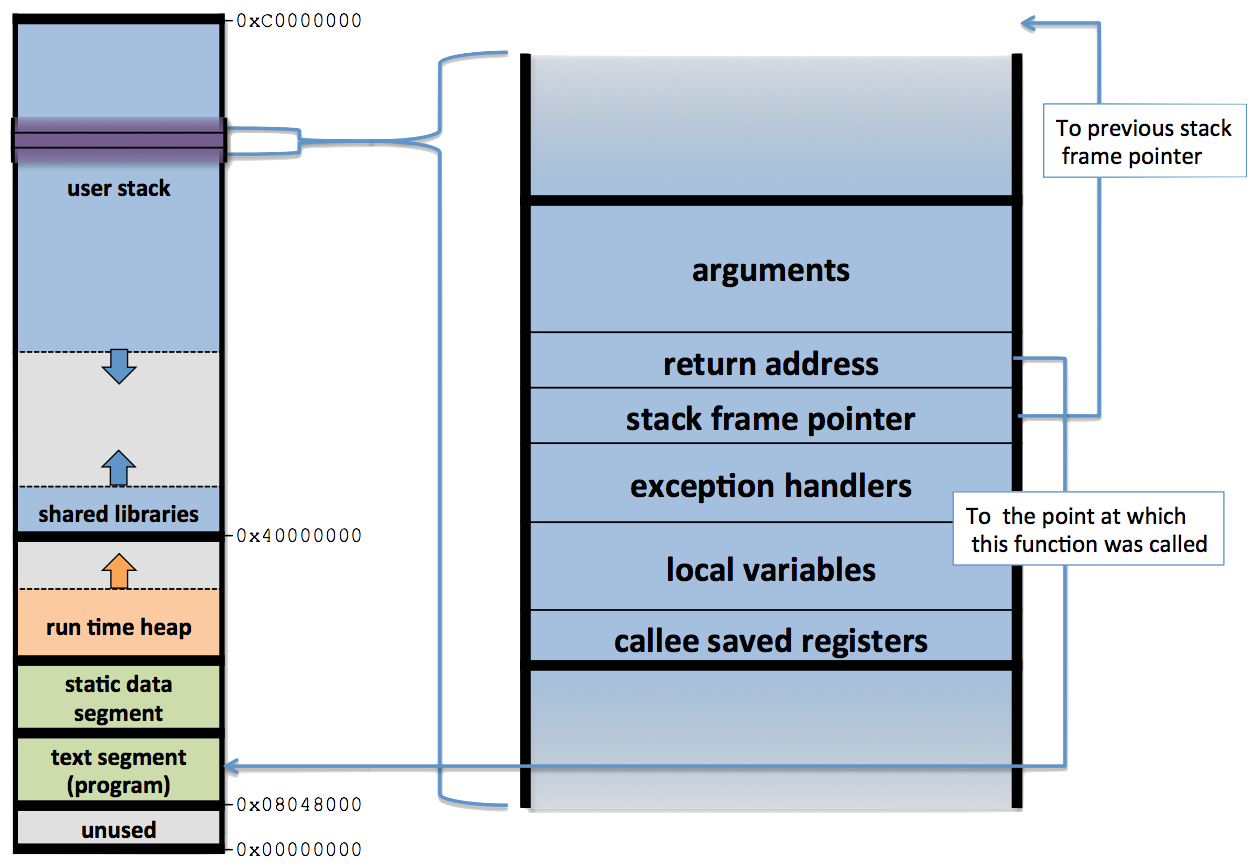
\includegraphics[scale=.3]{images/layout.png}
\end{center}

\begingroup
    \fontsize{6pt}{6pt}\selectfont
    \textbf{All of the following uses the IA-32 (Intel 32-bit systems) Notation.}\\
    Instructions are formatted at \verb|inst src dst|\\
    Memory addresses are 4 bytes long \\
    Registers are prefixed with \% \\
    Constants are prefixed with \$ \\
    (\$exx) means accessing memory at register \%exx \\
    l suffix for instructions that are 32-bit (long) instructions \\
    \textbf{SFP} is the saved \%ebp on the stack \\
    \textbf{OFP} is the old \%ebp from the previous stack frame \\
    \textbf{RIP} is the return address on the stack \\
    The \textbf{text} contains executable code of program \\
    The \textbf{heap} stores dynamically allocated data \\
    The \textbf{stack} stores local variables/info for each func call
\endgroup 

\subsubsection{Registers}
\textbf{General Purpose Registers} - \%eax, \%ebx, \%ecx, \%edx, \%edi, \%esi
(\%eax stores return value)

\textbf{\%ebp} - base pointer, indicates start of stack frame (gen const for given function).\\
\textbf{\%esp} - stack pointer, indicates bottom on stack (can and does change).\\
\textbf{\%eip} - instruction pointer, indicates instruction to run.\\


\subsubsection{Instructions}
\textbf{mov a, b} - copies value of a into b\\
\textbf{push a} - pushes a onto the stack (decrements stack, copies value over)\\
\textbf{pop a} - pop data from stack on a (copies value over and increments stack)\\
\textbf{call func} - pushes address of next instruction onto stack and transfers control to func\\
\textbf{ret} - pops return address of next instruction onto stack and transfers control to func\\
\textbf{leave} - mov \%ebp, \%esp then pop \%ebs (restores previous stack frame)\\
\textbf{pushl} \%ebp is part of the prologue for instructions that move the stack pointer to the current top of the stack. You then call movl \%esp, \%ebp to move \$ebp to where \%esp is. You do this at the beginning of each function call.\\
You push arguments in memory in reverse order.\\
Indexes in array are stored with the highest index immediately under the SFP (which is under the return address, and lower values under that.\\

\begingroup

\begin{center}
\vspace{-6pt}
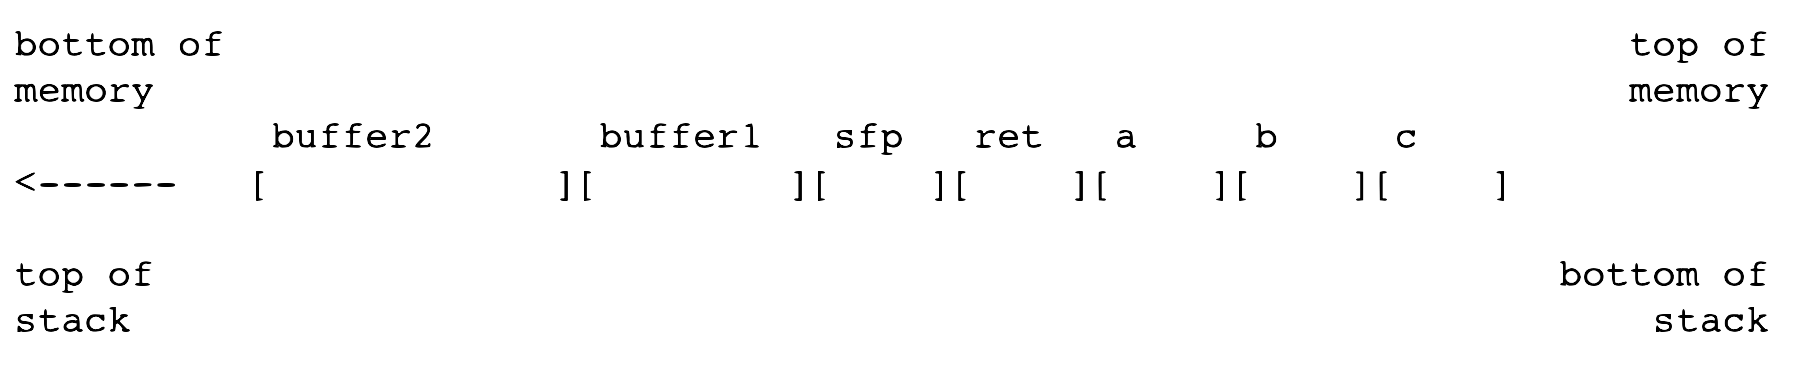
\includegraphics[scale=.25]{images/stack.png}
\end{center}
\vspace{-15pt}
\endgroup

\subsection*{C Specifics}
\begingroup
    \fontsize{6pt}{6pt}\selectfont
    \verb|char| is 1 byte, \verb|int| is 4 bytes, 1 byte is 8 bits\\

    \verb|void *memcpy(void *dest, const void *src, size_t n);| 
    \verb|size_t: typedef unsigned int size_t;|
    \verb|size_t fread(void *ptr, size_t size, size_t nmemb, FILE *stream)|
    Reads data from the given stream into the array pointed to, by ptr.\\

    \verb|strlen(s)| calculates the length of the string s, not including the terminating \verb|"\0"| character. \\
    \verb|strcpy(dst, src)| copies the string pointed to by src to dst, including the terminating \verb|"\0"| character \\
    \verb|strlcpy(dst, src, n)| avoids writing more than \verb|n| bytes into the buffer. \\
    \verb|sprintf| works exactly like \verb|printf|, but instead writes to the string pointed to by the first argument – terminates the characters written with a \verb|"\0"| \\
    \verb|snprintf(buf, sizeof buf, src)| is more secure than \verb|sprintf(buf, src)|. \\
    \verb|fgets(char str, int num, FILE *STREAM)| is more secure than \verb|gets()|. \\
    You can access an element before an array with a negative index.
\endgroup 

\subsection*{Buffer Overflows}

\subsubsection*{Simple Overflow}
An input with 80+ bytes will overflow \verb|buf|.
\begingroup
    \fontsize{6pt}{6pt}\selectfont
    \vspace{-8pt}
    \begin{verbatim}
    char buf[80];
    int (*fnptr)();
    void vulnerable() {
      gets(buf);
    }
    \end{verbatim}
    \vspace{-20pt}
\endgroup

% \subsubsection*{Malicious Code Injection}
% \begingroup
%     \fontsize{6pt}{6pt}\selectfont
%     \vspace{-1pt}
%     \begin{verbatim}
%     char buf[80];
%     int (*fnptr)();
%     void vulnerable() {
%       gets(buf); 
%     }
%     \end{verbatim}
%     \vspace{-20pt}
% \endgroup
% Attacker can overwrite frmptr with any address, redirecting program execution to other memory location

\subsubsection*{Stack Smashing}
Half of all technical attacks on operating systems that are reported come from memory overwritting attacks or smashing the stack. The basic idea behind it is that programmers are often careless about checking the size of arguments, so an attacker who passes a long argument to a program may find that some of it gets treated as code rather than data.
\begin{center}
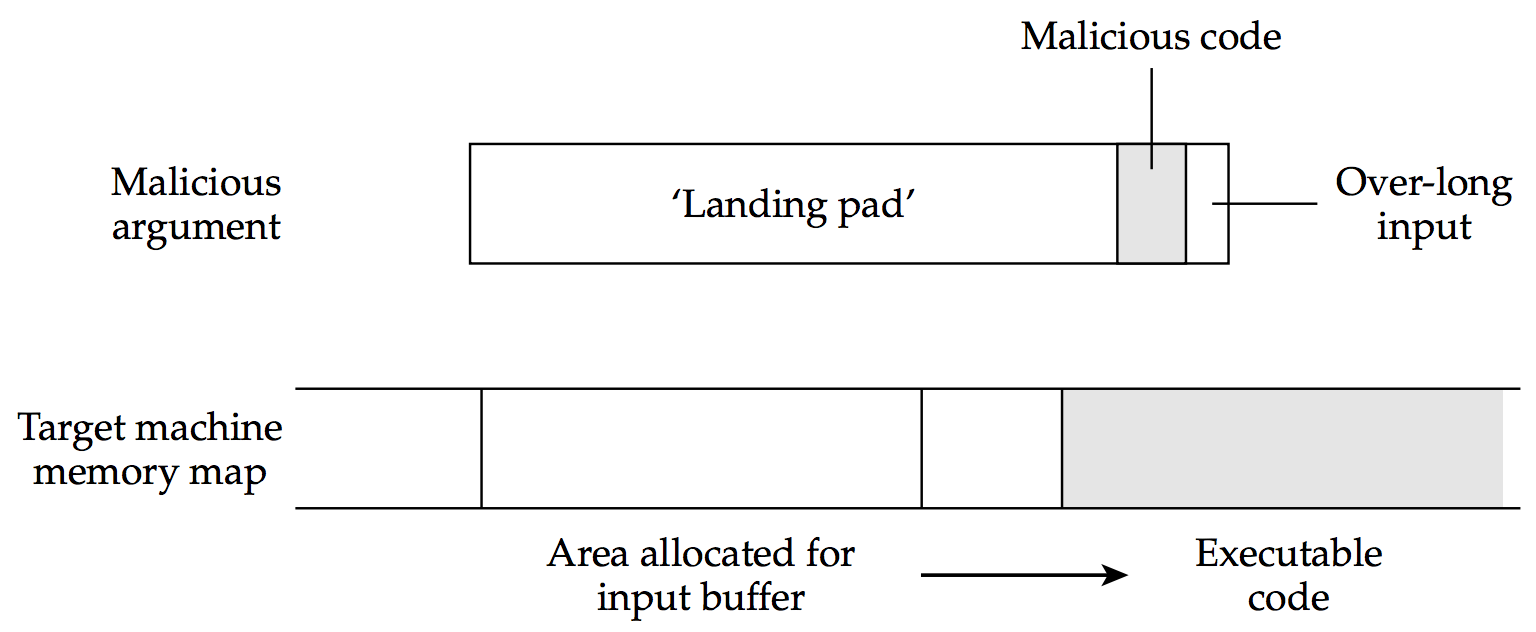
\includegraphics[scale=.25]{images/stack_smash.png}
\end{center}


\subsubsection*{Format String Vulnerability}
This arises when a machine accepts input data as a formatting instruction (ex \%n in the C command printf()). This can allow the string's author to write to the stack.
\begingroup
    \fontsize{6pt}{6pt}\selectfont
    \vspace{-1pt}
    \begin{verbatim}
    void vulnerable() {
        char buf[80];
        if (fgets(buf, sizeof buf, stdin) == NULL)
            return;
        printf(buf);
    }
    \end{verbatim}
    \vspace{-10pt}
\endgroup

Should be printf(“\%s”, buf). May crash/core dump. If attacker knows contects functions stack frame : \%x:\%x, reveals first two words of stack memory. \%x:\%s: treats next word as address and prints what is at that string.

\subsubsection*{Integer Conversion}
If you don't check for data sizes before writing, the integer manipulation attack uses an overflow, underflow, wrap-arround or truncation that can result from writing an inappropriate number of bytes to the stack. C will cast negative value to large pos integer \verb|memcpy()| will copy huge amount into \verb|buf| causing overflow

\begingroup
    \fontsize{6pt}{6pt}\selectfont
    \vspace{-1pt}
    \begin{verbatim}
    char buf[80];
    void vulnerable() {
        int len = read_int_from_network();
        char *p = read_string_from_network();
        if (len > 80) {
            error("length too large");
    return; }
        memcpy(buf, p, len);
    }
    \end{verbatim}
    \vspace{-10pt}
\endgroup


\subsection*{Defenses}

\textbf{Stack Canaries} places a random value on the stack before return address, and then checks to see if that values overwritten, and if it is, it raises an erro. 
\textbf{ASLR (Address Space Layout Randomization)} starts the stack at random place in memory rather than a fixed point the idea that if someone is using hardcoded malicious code, ASLR can get around it, but you can get around it by instead of return to a hardcode address, return a relative address (known address + offset to where you want to go) to where you are on the stack right now. 

In general make sure enough space is allocated, look for unchecked buffer writes, off-by-one errors (usually in indexing), inputs an attacker controls (they don't use a nullterminator or newline that you expect), malloc or calloc (initialized malloc) lengths. Keep tight bounds and restrictions for your program inputs. 

\textbf{Defensive programming} means each module takes responsibility for checking the validity of all inputs sent to it. Use libraries to automatically detect potential bugs. And use \textbf{Static Analysis} tools which scan for potential memory leaks. False negatives are better than false positives. If code does not trigger any warnings, then it is guaranteed to be free of bugs. \textbf{Runtime Checks} automatically inject checks everywhere there is a chance of exploitation, which slows you down (10–150\%) and can be tedious to run on legacy code. 

\begingroup
    \fontsize{6pt}{6pt}\selectfont
    \vspace{-6pt}
    \begin{verbatim}
    char digit_to_char(int i) { // BETTER
            char convert[] = "0123456789";
            if (i < 0 || i > 9)     # Check array access bounded
                return "?"; // or, call exit()
            return convert[i];
    \end{verbatim}
    \vspace{-15pt}
\endgroup

\subsection*{Fuzz Testing}

\textbf{Random}
Given nothing, input into the program random values and see where it crashes. \\
\textbf{Mutational}
Given a template as input, modify stuff (like bits) and run, to figure out which values can cause problems. \\
\textbf{Generational}
Given some constraints, and fuzz those value to figure out which can cause problems. 


%%%%%%%%%%%%%%%%%%%%%%%%%


\section*{Security Methodologies}




%%%%%%%%%%%%%%%%%%%%%%%%%


\section*{Software Security}
We want our systems to maintain \textbf{Confidentiality}, \textbf{Integrity}, and \textbf{Availability}.


\textbf{Leveraging Modularity} (privilege separation) is strengthening security by providing forms of isolation that is keeping potential problems localized, and minimizing the assumptions made between components.

\textbf{Threat Models} are the environments and context in which your security was designed. As time goes on they have a knack for changing, like what happened to the Internet (University Network to Now).

\textbf{Kerkhoff's Principle} is that Cryptosystems should remain secure even when the attacker knows all internal details of the system. The key should be the only thing that must be kept secret, and the system should
be designed to make it easy to change keys that are leaked (or suspected to be leaked). Changing the key is easier than replacing software.

% \textbf{Defense in Depth} is the idea behind this is to put layers of security so that even if one of them fails, the others maintain the integrity of the system. For example 


% \subsubsection*{Preconditons}

% \subsubsection*{Postcondtions}


\subsection*{Access Control}
A \textit{Subject} tries to access an \textit{Object} as is restricted by the \textit{Policy}.\\
\textbf{Authorization} is who should be able to perform which actions. \textbf{Authentication} is verifying who is requesting the action. An \textbf{Audit} is a log of all the actions, so that there is \textbf{Accountability} to hold people to their actions. 

In web we can have have \textbf{Centralized Enforcement} where the database centrally checks policy for each access. There is also \textbf{Integrated Access Control} which verifies the policy wherever there is data access. It is more flexible but perhaps more prone to error.

% \subsubsection*{Access Control Matrix}
% \begin{tabular}{|l|l|l|l|l|}
%     \hline
%     & Asset 1 & Asset 2 & file & device\\
%     \hline
%     \hline
%     Role 1 & read,write,execute,own & execute & read & write\\
%     \hline
%     Role 2 & read & read,execute & & \\
%     \hline
% \end{tabular}

% \subsubsection*{Simple Access Control List}
% \begin{center}
% \begin{tabular}{|l|c|}
% \hline
% User & Accounting Data\\
% \hline
% Sam & rw\\
% Alice & rw\\
% Bob & r\\
% \hline
% \end{tabular}
% \end{center}


\subsection*{Trusted Computing Base}
This is the minimum set of components to ensure security. TCB is one that is able to violate our security goals if it misbehaves. Ensure the security of your TCB. TCB must be large enough so that nothing outside the TCB can violate security. For example Authorized users allowed to enter system using SSH so the TCB is the SSH daemon, Operating System, CPU. A \textbf{Reference Monitor} is TCB specialized for access control. Design Principles for TCB are \textbf{Unbypassable} - no way to breach system security by bypass TCB (you have complete mediation), \textbf{Tamper-resistant} - protected from tampering from other systems and \textbf{Verifiable} - verify the correctness of the TCB. Use \textbf{Least Privilege} to only give each part of the system the minimum amount of access rights needed. Smaller systems are easier to secure. Isolate privileges to specific components as much as possible. 

\subsubsection*{Race Conditions}
Race conditions occur when a transaction is carried out in two or more stages, and it is possible for someone to alter it after the stage which involves verifying access rights.

\subsection*{TOCTTOU Vulnerability}
Time-Of-Check To Time-Of-Use is a issue that arises when meaning of variable changed from the time when it is checked and the time when it is used such as in UNIX filesystem calls. Can arise anywhere there is mutable state that is shared between two or more entities.

\subsection*{Core Ideas}
\textbf{Security relies on the economic constraints}, \textbf{Design security from the start}, give the \textbf{Least Privileges} possible, have \textbf{Fail Safe Defaults}, \textbf{Layer Security}, Ensure people \textbf{psychologically} accept security (shitty passwords), go for \textbf{Complete Mediation} (end to end control), know and track your \textbf{Threat Model}, ensure that if you can't protect you can at least \textbf{Detect} vulnerabilities, don't rely on \textbf{Obscurity} to keep your system safe, assume \textbf{system architecture} is known, try to plan for the \textbf{Worse Case} and \textbf{Study Attacks}. You are only as secure as the weakest link.


%%%%%%%%%%%%%%%%%%%%%%%%%

\section*{Web Security}

The web allows for sharing applications and information between a client (your browser) and a source (a web server). One of the main ways to do this is through HTTP (Hypertext Transfer Protocol). The allows you to send requests and get responses. \\

URL (Uniform Resource Locator) such as \url{http://atrus.co:2000/fg?search=security#web} is separated into \url{protocol://hostname.tld:port/path?query#fragment} \\

HTML + CSS + JS = DOM --Painter--> Bitmap \\

The web is a good example of \textbf{bolt-on security}. Security model was added later. 

We want \textbf{Integrity} where no malicious site should tamper with my computer of info on other sites (Sandbox JS, Access Control, Updates), \textbf{Confidentiality} none of my confidential info should be given to malicious sites (Same Origin Policy), and \textbf{Privacy} where malicious websites should not be able to spy on me or my activities. 


\subsection*{Same Origin Policy}
Stipulates that each site is isolated from other sites, where origin is protocol + hostname + port. One origin should no be able to access he resources of another origin. Cross origin communication is allowed through a API called \verb|postMessage| where the receiving origin see the message's origin and can accept or deny message. 

\subsection*{SQL Injection}
These commonly arise when a careless web developer passes user input to a back-end database without checking to see whether it contains SQL code and doesn't escape \verb|'+-;|. You can get around it using frameworks such as ParameterizedSQL that sanitize input. You can also use \textbf{Prepared Statements} which are preset allowed commands. Exploits like the following allow you to see or remove all the users.
\begingroup
    \fontsize{6pt}{6pt}\selectfont
    \vspace{-5pt}
    \begin{verbatim}
    ok = execute(SELECT ... where user=' ' or 1=1 --)
    ok = execute(SELECT ... where user=' '; DROP TABLE Users)
    \end{verbatim}
    \vspace{-16pt}
\endgroup

\subsection*{Cookies}
Since good HTTP is stateless (no info is maintained between requests and requests are independent), we use cookies. Browser stores cookies that web sites ask to store a set of key value pairs such as (domain, when to send), (path, when to send), (secure, SSL), (expires, time). \textbf{HTTPOnly} attribute means no JS access. Cookies can be accessed by parent domains (except TLD), but they cannot set cookies for their subdomains.
% but subdomains can \textit{read} but not \textit{set} cookies for parent domains. \\
Sessions allow you do set a time period for authentication and are tied to user. Tokens are generated by the server for a set tie period. Session Cookies send the cookie with every request and are thus vulnerable to CSRF, putting the token in URL can leak the token, and putting it in hidden form fields only work for short sessions. Thus we use a combination of these for optimal effect. 

\subsection*{Privacy}
A third party cookie, say from an advertiser that has a relationship with a website, can follow your activity and thus form a trail of you. Google Analytics sends a ton of data from websites to their platform. Facebook can track all the sites you are on if that site has a like button. This all makes Internet content free (ads), but there is concern how easy it is to get your data and we don't know how it can be misused. Plus you don't really know what you are giving away (image location data). Don't trust private browsing, cookies are still used within session. 

\subsection*{Cross Site Scripting (XSS)}
Very common web vulnerability. Same origin policy does not protect against XSS. Two main types:
\begin{itemize}
\item \textbf{Stored XSS} is when an attacker leaves malicious JS on a server that is then sent to a client (subverts SOP) which then does something malicious to the client. For example executing a URL that sends me money through a request. You can steal cookies and operate on session cookies. Example is storing HTML/JS on a Database that doesn't escape it like Samy's MySpace worm. 
\item \textbf{Reflected XSS} is when a user is tricked into clicking a malicious link, submitting a specially crafted form, or browsing to a malicious site, the injected code travels to the vulnerable website and the web service reflects it back. For example stealing a cookie by "searching" a script that requests it form the server (\verb|document.cookie|) and sends it. This works when there is no form validation (such as escaping HTML tags).
\end{itemize}

You can protect against these by having a whitelist of accepted scripts (CSP) and disallowing all other scripts. Use proper form validation. 


\subsection*{Cross-Site Request Forgery (CSRF)}
Is when a session cookies remains in browser state after a user successfully authenticates. Malicious scripts from specific sites can ask for the cookie and forge requests with full authentication (such as sending money using a payment service). To combat this we use \textbf{secret validation tokens} (secret tokens that server looks for to make sure request is coming from authorized source). Often we use the user's \textbf{session ID} for validation, but an attacker can impersonate these if they can see the content of the page. We can also use a \textbf{nonce} (single purpose random number) that is sent with cookie and is hidden but they can be replaced by an attackers CSRF token. Else we can use a \textbf{session dependent nonce} which binds the user's CSRF token to their session ID, but this requires the server to maintain a table of these pairs.\\
\textbf{Referrer validation} is when includes a referrer header that indicates where the request came from. This can be used to differentiate cross site requests. You have to set the tolerance for which referers to allow. There are also privacy concerns with being able to see referer header URL such as search queries. 
\textbf{Custom Headers} allow for sites to send headers amongst themselves, and since they are custom they don't even need cookies values, the server just has to reject requests without the custom header. They are limitations, such as data export format and it not working across domains. 

\subsection*{Authentication}
Server should authenticate client (Passwords, Key, Fingerprint) and client should authenticate web servers (Certificates). Two-factor authentication is using two of (Knowledge, Possession, Attributes). After authecication as session cookie with my session ID is stored on my browser and the webserver maintains a list of active sessions. HTTP uses the cookie to authenticate every request automatically. Vulnerable to CSRF attacks. \\

\textbf{Phishing} is when an attacker fakes a site to trick a user into giving up their credentials or data. Prevent this by checking the URL and certificate. Don't click on unknown links. 

\subsection*{UI Exploitation}
\textbf{Clickjacking} is creating a link that seem sto link to one website, but with some tricky (usually using JS) can do things like like something on Facebook or redirect to another URL. 

\textbf{iframes} can be used to link one website within another, which can cause one site to appear like the normal one but can have a layer of maliciousness on it such as stealing userid and password. Frames follow same origin so you can't run malicious JS on the content of the frame, but you can use clickjacking to add a partial overlay to make it seem like you are entering your info in the right place. 

This compromises the \textbf{visual integrity} of the page (things look different than they are). You can also use fake cursors to trick users into clicking the wrong thing. User confirmation while bad UX helps to alleviate these attacks. UI Randomizations are good as well but are susceptible to multi-click attacks. Removing cursor customization (16\% attack rate), freezing screen around the pointer (4\%), adding a lightbox (3\%), or delay (1\%), or disabling clicks unless pointer is over target (0\%). 

\textbf{Framebusting} is code on a website that prevents other sites from framing it, usually with a conditional statement and a counter action such as \verb|if (top != self) { top.location = self.location; }|. However these are often defeated due to small bugs in the framebusting code (like not using HTTPS) or with a XSS filter that removes the scripts from the page. We can also use X-Frame-Options which either deny rendering in framed context or only render if the top frame is the same origin as framed page.


%%%%%%%%%%%%%%%%%%%%%%%%%


\section*{Cryptography}
\textbf{Confidentiality} Prevent adversaries reading data, \textbf{Integrity} prevent attackers from altering some data, \textbf{Authenticity} determines who created a given document.

\subsection*{Attacks}
\begingroup
    \fontsize{6pt}{6pt}\selectfont
    \textbf{Ciphertext Only} is Eve intercept encrypted message and wants to recover plaintext. \\ 
    \textbf{Known Plaintext} is when Eve intercept encrypt msg and has partial info about plaintext \\ 
    \textbf{Chosen Plaintext} is when Eve trick Alice to encrypt messages $M_1, M_2, \ldots, M_n$ of Eve’s choice. Eve can observe the resulting ciphertexts. Try to recover new message M. \\
    \textbf{Chosen Ciphertext} is when Eve can trick Bob into decrypting some ciphertexts $C_1, \ldots, C_n$ and then use this to learn decryption of some other ciphertext $C$. Combining the last two is a very serious threat. 
\endgroup

\begingroup
    \fontsize{6pt}{6pt}\selectfont
    \textbf{Block Ciphers} \textbf{Encrypt} with $E_{K}(M) = E(K,M);$ \textbf{Decrypt} with $D_K(E_K(M)) = M$\\

    \textbf{Symmetric Key Crypto} is where the same secret key us used by sender and receiver and is reusable, it is built on block ciphers. \\

    \textbf{Public Key Crypto} is where sender and receiver use different keys. \\

    \textbf{One-Time Pad (OTP)} can only be used once. Alice and Bob share n-bit secret key. (XOR of the same bit is 0 and different bits is 1) \textbf{Encrypt} with $c_j = m_j \oplus k_j$. \textbf{Decrypting} is done with $m_j = c_j \oplus k_j$ 
\endgroup

\begingroup
\begin{center}
\vspace{-6pt}
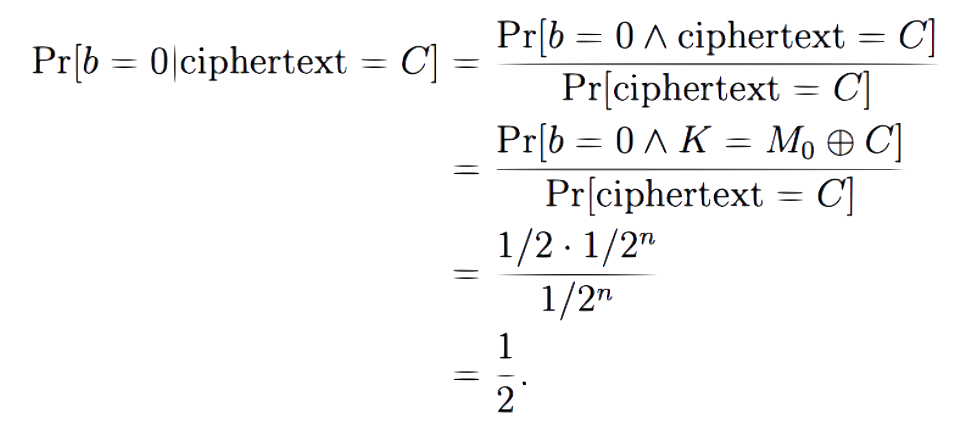
\includegraphics[scale=.25]{images/proof.png}
\end{center}
\vspace{-15pt}
\endgroup

% \subsection*{Symmetric Key Encryption}





%\rule{0.3\linewidth}{0.1pt}
\scriptsize

\end{multicols}
\end{document}
